\documentclass[a4paper, oneside,11pt]{article}
\usepackage[a4paper,top=3cm,bottom=3cm,left=3cm,right=3cm,marginparwidth=1.75cm]{geometry}
\usepackage[utf8]{inputenc}
\usepackage{lipsum}
\usepackage{graphicx}
\usepackage{times}
\usepackage{xcolor}
%\usepackage{booktabs}
\usepackage{float}
\usepackage{color}
\usepackage{hyperref}
\usepackage{amsmath}
%\usepackage{subfig}
\usepackage{subcaption}
\usepackage[backend=biber,
    style=numeric,sorting=none]{biblatex}
\addbibresource{ref.bib}
\hypersetup{
    colorlinks=true,
    linkcolor=blue,
    urlcolor=blue,
}
\graphicspath{{/}}
\usepackage{adjustbox}
\usepackage{tabularx}
\usepackage{multirow}
\usepackage{titlesec}
\usepackage{graphicx}
\usepackage{upgreek}
\usepackage{enumitem}  
\usepackage{comment} 
\usepackage{upgreek}
%%%%%%%%%%%%%%%%%%%%%%%%%%%%%%%%%%%%%%%%%%%%%%%%%%%%%%%%%%%%%%%%%%%%

\begin{document}

\begin{table}[h]
		\begin{adjustbox}{width = \linewidth}
			\begin{tabular}{c c c}
				\multirow{5}{*}{ 
\includegraphics[width=0.13\textwidth]{iitb_logo.png}} \hfill &  \large{{Student Satellite Project}}  & \hfill \multirow{5}{*}{ 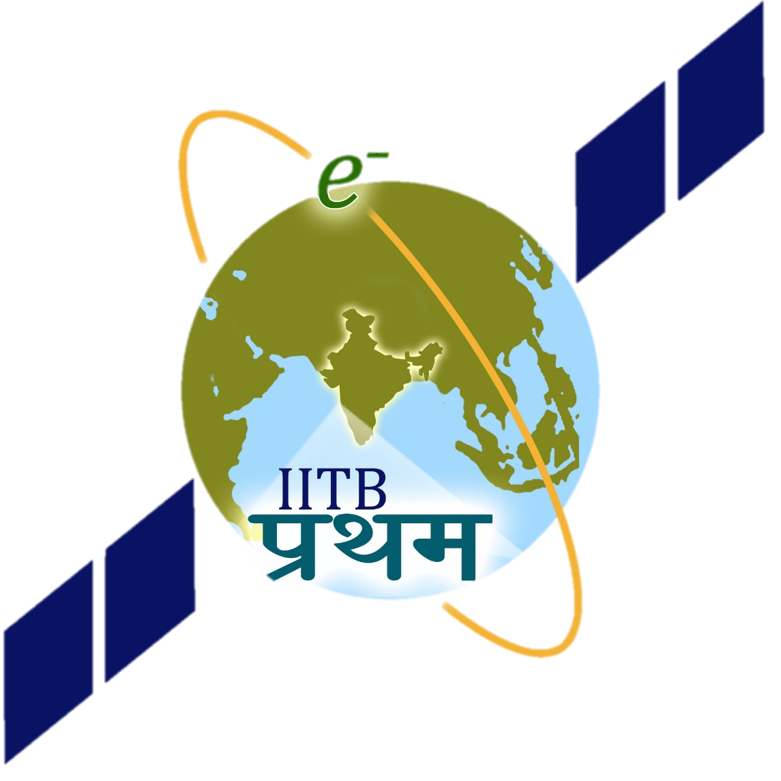
\includegraphics[width=0.13\textwidth]{pratham_logo.png}} \\
				& {Indian Institute of Technology, Bombay} &\\
				& {Powai, Mumbai - 400076, INDIA} &\\
				&{} &\\
				& Website: {www.aero.iitb.ac.in/satlab} &\\
				\\
				&\large{\textbf{Readme file for TLE2OrbitElements.py}}&\\
				&Attitude Determination and Control Subsystem&\\
				\hline
			\end{tabular}
		\end{adjustbox}
\end{table}
\section*{}
\textbf{Author: Sumit Agrawal}\\
\textbf{Date:08 July 2018}\\
This code is convert the given Two Line Element (TLE) into orbital elements.\\
Input: Two Line Element. \\ Do not copy paste the TLE from some other source like (n2yo.com). If you do make sure you rewrite the signs(+,-) as python sometimes do not understand signs(some syntex error).\\
Output:Orbital Elements \{Inclination (degrees),Right ascension of the ascending node (degrees), Eccentricity, Argument of perigee (degrees) ,Mean Anomaly (degrees),Mean Motion (revolutions per day) \}; First time derivative of mean motion;  Second time derivative of mean motion; Bstar; Epoach year; Epoach and  other parameter {Satellite No., Class No., International designator}\\

References: \url{https://en.wikipedia.org/wiki/Two-line_element_set}


\printbibliography 
\end{document}
